% Options for packages loaded elsewhere
\PassOptionsToPackage{unicode}{hyperref}
\PassOptionsToPackage{hyphens}{url}
%
\documentclass[
  5pt,
  ignorenonframetext,
]{beamer}
\usepackage{pgfpages}
\setbeamertemplate{caption}[numbered]
\setbeamertemplate{caption label separator}{: }
\setbeamercolor{caption name}{fg=normal text.fg}
\beamertemplatenavigationsymbolsempty
% Prevent slide breaks in the middle of a paragraph
\widowpenalties 1 10000
\raggedbottom
\setbeamertemplate{part page}{
  \centering
  \begin{beamercolorbox}[sep=16pt,center]{part title}
    \usebeamerfont{part title}\insertpart\par
  \end{beamercolorbox}
}
\setbeamertemplate{section page}{
  \centering
  \begin{beamercolorbox}[sep=12pt,center]{part title}
    \usebeamerfont{section title}\insertsection\par
  \end{beamercolorbox}
}
\setbeamertemplate{subsection page}{
  \centering
  \begin{beamercolorbox}[sep=8pt,center]{part title}
    \usebeamerfont{subsection title}\insertsubsection\par
  \end{beamercolorbox}
}
\AtBeginPart{
  \frame{\partpage}
}
\AtBeginSection{
  \ifbibliography
  \else
    \frame{\sectionpage}
  \fi
}
\AtBeginSubsection{
  \frame{\subsectionpage}
}
\usepackage{lmodern}
\usepackage{amssymb,amsmath}
\usepackage{ifxetex,ifluatex}
\ifnum 0\ifxetex 1\fi\ifluatex 1\fi=0 % if pdftex
  \usepackage[T1]{fontenc}
  \usepackage[utf8]{inputenc}
  \usepackage{textcomp} % provide euro and other symbols
\else % if luatex or xetex
  \usepackage{unicode-math}
  \defaultfontfeatures{Scale=MatchLowercase}
  \defaultfontfeatures[\rmfamily]{Ligatures=TeX,Scale=1}
\fi
\usetheme[]{Berlin}
\usecolortheme{beaver}
\usefonttheme{structurebold}
% Use upquote if available, for straight quotes in verbatim environments
\IfFileExists{upquote.sty}{\usepackage{upquote}}{}
\IfFileExists{microtype.sty}{% use microtype if available
  \usepackage[]{microtype}
  \UseMicrotypeSet[protrusion]{basicmath} % disable protrusion for tt fonts
}{}
\makeatletter
\@ifundefined{KOMAClassName}{% if non-KOMA class
  \IfFileExists{parskip.sty}{%
    \usepackage{parskip}
  }{% else
    \setlength{\parindent}{0pt}
    \setlength{\parskip}{6pt plus 2pt minus 1pt}}
}{% if KOMA class
  \KOMAoptions{parskip=half}}
\makeatother
\usepackage{xcolor}
\IfFileExists{xurl.sty}{\usepackage{xurl}}{} % add URL line breaks if available
\IfFileExists{bookmark.sty}{\usepackage{bookmark}}{\usepackage{hyperref}}
\hypersetup{
  pdftitle={Seminar},
  hidelinks,
  pdfcreator={LaTeX via pandoc}}
\urlstyle{same} % disable monospaced font for URLs
\newif\ifbibliography
\usepackage{graphicx}
\makeatletter
\def\maxwidth{\ifdim\Gin@nat@width>\linewidth\linewidth\else\Gin@nat@width\fi}
\def\maxheight{\ifdim\Gin@nat@height>\textheight\textheight\else\Gin@nat@height\fi}
\makeatother
% Scale images if necessary, so that they will not overflow the page
% margins by default, and it is still possible to overwrite the defaults
% using explicit options in \includegraphics[width, height, ...]{}
\setkeys{Gin}{width=\maxwidth,height=\maxheight,keepaspectratio}
% Set default figure placement to htbp
\makeatletter
\def\fps@figure{htbp}
\makeatother
\setlength{\emergencystretch}{3em} % prevent overfull lines
\providecommand{\tightlist}{%
  \setlength{\itemsep}{0pt}\setlength{\parskip}{0pt}}
\setcounter{secnumdepth}{-\maxdimen} % remove section numbering
\usepackage[orientation = landscape, size = custom, width = 16, height = 9, scale = 0.5]{beamerposter}
\setbeamertemplate{footline}[frame number]
\usefonttheme{serif}
% ## ---------------------------------------------------------------------- 
% \setbeamerfont{supervisor}{size = \scriptsize}
% \setbeamerfont{instructor}{size = \scriptsize}
% ## ---------------------------------------------------------------------- 
\defbeamertemplate{title page}{RunTemplate}
{
  \vfill
  % ## ---------------------------------------------------------------------- 
  \begin{beamercolorbox}[sep = 10pt, center]{titleGraph}
    \inserttitlegraphic
  \end{beamercolorbox}
  % ## ---------------------------------------------------------------------- 
  \begin{beamercolorbox}[sep = 8pt, center, rounded = true]{title}
    \usebeamerfont{title}\inserttitle\par
    \ifx\insertsubtitle\@empty
  \else
  {\usebeamerfont{subtitle}\usebeamercolor[fg]{subtitle}\insertsubtitle\par}
  \fi
  \end{beamercolorbox}
  % ## ---------------------------------------------------------------------- 
  \vskip0.4em
  % ## ---------------------------------------------------------------------- 
  \begin{beamercolorbox}[sep = 8pt, center]{author}
    \usebeamerfont{author}\insertauthor\par
  \end{beamercolorbox}
  % ## ---------------------------------------------------------------------- 
  % \begin{beamercolorbox}[sep = 5pt, center]{supervisor}
    % \usebeamerfont{supervisor}Supervisor: \supervisor
  % \end{beamercolorbox}
  % ## ---------------------------------------------------------------------- 
  % \begin{beamercolorbox}[sep = 5pt, center]{instructor}
    % \usebeamerfont{instructor}\instructor
  % \end{beamercolorbox}
  % ## ---------------------------------------------------------------------- 
  \begin{beamercolorbox}[sep = 8pt, center]{institute}
    \usebeamerfont{institute}\insertinstitute\par
  \end{beamercolorbox}
  % ## ---------------------------------------------------------------------- 
  \begin{beamercolorbox}[sep = 8pt, center]{date}
    \usebeamerfont{date}\insertdate\par
  \end{beamercolorbox}
  \vfill
}
\setbeamertemplate{title page}[RunTemplate]

\newenvironment{cols}[1][]{}{}

\newenvironment{col}[1]{\begin{minipage}{#1}\ignorespaces}{%
\end{minipage}
\ifhmode\unskip\fi
\aftergroup\useignorespacesandallpars}

\def\useignorespacesandallpars#1\ignorespaces\fi{%
#1\fi\ignorespacesandallpars}

\makeatletter
\def\ignorespacesandallpars{%
  \@ifnextchar\par
    {\expandafter\ignorespacesandallpars\@gobble}%
    {}%
}
\makeatother
\AtBeginEnvironment{longtable}{\tiny} \titlegraphic{\centering 
\includegraphics{./logo_lixiao.png}} \usepackage{caption} \captionsetup{font={tiny}} \usepackage{setspace} \setstretch{1.3} \linespread{1.3} \usepackage{xeCJK}

\title{Seminar}
\author{Lichuang Huang}
\date{2023-12-16}
\institute{Wie-Biotech}

\begin{document}
\frame{\titlepage}

\hypertarget{tasks-summary}{%
\section{Tasks summary}\label{tasks-summary}}

\begin{frame}[fragile]{Overview}
\protect\hypertarget{overview}{}
\begin{verbatim}
## Warning in grid.Call.graphics(C_text, as.graphicsAnnot(x$label), x$x, x$y, : conversion failure on '备单业务 (9.4%)' in
## 'mbcsToSbcs': dot substituted for <e5>
\end{verbatim}

\begin{verbatim}
## Warning in grid.Call.graphics(C_text, as.graphicsAnnot(x$label), x$x, x$y, : conversion failure on '备单业务 (9.4%)' in
## 'mbcsToSbcs': dot substituted for <a4>
\end{verbatim}

\begin{verbatim}
## Warning in grid.Call.graphics(C_text, as.graphicsAnnot(x$label), x$x, x$y, : conversion failure on '备单业务 (9.4%)' in
## 'mbcsToSbcs': dot substituted for <87>
\end{verbatim}

\begin{verbatim}
## Warning in grid.Call.graphics(C_text, as.graphicsAnnot(x$label), x$x, x$y, : conversion failure on '备单业务 (9.4%)' in
## 'mbcsToSbcs': dot substituted for <e5>
\end{verbatim}

\begin{verbatim}
## Warning in grid.Call.graphics(C_text, as.graphicsAnnot(x$label), x$x, x$y, : conversion failure on '备单业务 (9.4%)' in
## 'mbcsToSbcs': dot substituted for <8d>
\end{verbatim}

\begin{verbatim}
## Warning in grid.Call.graphics(C_text, as.graphicsAnnot(x$label), x$x, x$y, : conversion failure on '备单业务 (9.4%)' in
## 'mbcsToSbcs': dot substituted for <95>
\end{verbatim}

\begin{verbatim}
## Warning in grid.Call.graphics(C_text, as.graphicsAnnot(x$label), x$x, x$y, : conversion failure on '备单业务 (9.4%)' in
## 'mbcsToSbcs': dot substituted for <e4>
\end{verbatim}

\begin{verbatim}
## Warning in grid.Call.graphics(C_text, as.graphicsAnnot(x$label), x$x, x$y, : conversion failure on '备单业务 (9.4%)' in
## 'mbcsToSbcs': dot substituted for <b8>
\end{verbatim}

\begin{verbatim}
## Warning in grid.Call.graphics(C_text, as.graphicsAnnot(x$label), x$x, x$y, : conversion failure on '备单业务 (9.4%)' in
## 'mbcsToSbcs': dot substituted for <9a>
\end{verbatim}

\begin{verbatim}
## Warning in grid.Call.graphics(C_text, as.graphicsAnnot(x$label), x$x, x$y, : conversion failure on '备单业务 (9.4%)' in
## 'mbcsToSbcs': dot substituted for <e5>
\end{verbatim}

\begin{verbatim}
## Warning in grid.Call.graphics(C_text, as.graphicsAnnot(x$label), x$x, x$y, : conversion failure on '备单业务 (9.4%)' in
## 'mbcsToSbcs': dot substituted for <8a>
\end{verbatim}

\begin{verbatim}
## Warning in grid.Call.graphics(C_text, as.graphicsAnnot(x$label), x$x, x$y, : conversion failure on '备单业务 (9.4%)' in
## 'mbcsToSbcs': dot substituted for <a1>
\end{verbatim}

\begin{verbatim}
## Warning in grid.Call.graphics(C_text, as.graphicsAnnot(x$label), x$x, x$y, : conversion failure on '固定业务 (37.5%)' in
## 'mbcsToSbcs': dot substituted for <e5>
\end{verbatim}

\begin{verbatim}
## Warning in grid.Call.graphics(C_text, as.graphicsAnnot(x$label), x$x, x$y, : conversion failure on '固定业务 (37.5%)' in
## 'mbcsToSbcs': dot substituted for <9b>
\end{verbatim}

\begin{verbatim}
## Warning in grid.Call.graphics(C_text, as.graphicsAnnot(x$label), x$x, x$y, : conversion failure on '固定业务 (37.5%)' in
## 'mbcsToSbcs': dot substituted for <ba>
\end{verbatim}

\begin{verbatim}
## Warning in grid.Call.graphics(C_text, as.graphicsAnnot(x$label), x$x, x$y, : conversion failure on '固定业务 (37.5%)' in
## 'mbcsToSbcs': dot substituted for <e5>
\end{verbatim}

\begin{verbatim}
## Warning in grid.Call.graphics(C_text, as.graphicsAnnot(x$label), x$x, x$y, : conversion failure on '固定业务 (37.5%)' in
## 'mbcsToSbcs': dot substituted for <ae>
\end{verbatim}

\begin{verbatim}
## Warning in grid.Call.graphics(C_text, as.graphicsAnnot(x$label), x$x, x$y, : conversion failure on '固定业务 (37.5%)' in
## 'mbcsToSbcs': dot substituted for <9a>
\end{verbatim}

\begin{verbatim}
## Warning in grid.Call.graphics(C_text, as.graphicsAnnot(x$label), x$x, x$y, : conversion failure on '固定业务 (37.5%)' in
## 'mbcsToSbcs': dot substituted for <e4>
\end{verbatim}

\begin{verbatim}
## Warning in grid.Call.graphics(C_text, as.graphicsAnnot(x$label), x$x, x$y, : conversion failure on '固定业务 (37.5%)' in
## 'mbcsToSbcs': dot substituted for <b8>
\end{verbatim}

\begin{verbatim}
## Warning in grid.Call.graphics(C_text, as.graphicsAnnot(x$label), x$x, x$y, : conversion failure on '固定业务 (37.5%)' in
## 'mbcsToSbcs': dot substituted for <9a>
\end{verbatim}

\begin{verbatim}
## Warning in grid.Call.graphics(C_text, as.graphicsAnnot(x$label), x$x, x$y, : conversion failure on '固定业务 (37.5%)' in
## 'mbcsToSbcs': dot substituted for <e5>
\end{verbatim}

\begin{verbatim}
## Warning in grid.Call.graphics(C_text, as.graphicsAnnot(x$label), x$x, x$y, : conversion failure on '固定业务 (37.5%)' in
## 'mbcsToSbcs': dot substituted for <8a>
\end{verbatim}

\begin{verbatim}
## Warning in grid.Call.graphics(C_text, as.graphicsAnnot(x$label), x$x, x$y, : conversion failure on '固定业务 (37.5%)' in
## 'mbcsToSbcs': dot substituted for <a1>
\end{verbatim}

\begin{verbatim}
## Warning in grid.Call.graphics(C_text, as.graphicsAnnot(x$label), x$x, x$y, : conversion failure on '其他业务 (53.1%)' in
## 'mbcsToSbcs': dot substituted for <e5>
\end{verbatim}

\begin{verbatim}
## Warning in grid.Call.graphics(C_text, as.graphicsAnnot(x$label), x$x, x$y, : conversion failure on '其他业务 (53.1%)' in
## 'mbcsToSbcs': dot substituted for <85>
\end{verbatim}

\begin{verbatim}
## Warning in grid.Call.graphics(C_text, as.graphicsAnnot(x$label), x$x, x$y, : conversion failure on '其他业务 (53.1%)' in
## 'mbcsToSbcs': dot substituted for <b6>
\end{verbatim}

\begin{verbatim}
## Warning in grid.Call.graphics(C_text, as.graphicsAnnot(x$label), x$x, x$y, : conversion failure on '其他业务 (53.1%)' in
## 'mbcsToSbcs': dot substituted for <e4>
\end{verbatim}

\begin{verbatim}
## Warning in grid.Call.graphics(C_text, as.graphicsAnnot(x$label), x$x, x$y, : conversion failure on '其他业务 (53.1%)' in
## 'mbcsToSbcs': dot substituted for <bb>
\end{verbatim}

\begin{verbatim}
## Warning in grid.Call.graphics(C_text, as.graphicsAnnot(x$label), x$x, x$y, : conversion failure on '其他业务 (53.1%)' in
## 'mbcsToSbcs': dot substituted for <96>
\end{verbatim}

\begin{verbatim}
## Warning in grid.Call.graphics(C_text, as.graphicsAnnot(x$label), x$x, x$y, : conversion failure on '其他业务 (53.1%)' in
## 'mbcsToSbcs': dot substituted for <e4>
\end{verbatim}

\begin{verbatim}
## Warning in grid.Call.graphics(C_text, as.graphicsAnnot(x$label), x$x, x$y, : conversion failure on '其他业务 (53.1%)' in
## 'mbcsToSbcs': dot substituted for <b8>
\end{verbatim}

\begin{verbatim}
## Warning in grid.Call.graphics(C_text, as.graphicsAnnot(x$label), x$x, x$y, : conversion failure on '其他业务 (53.1%)' in
## 'mbcsToSbcs': dot substituted for <9a>
\end{verbatim}

\begin{verbatim}
## Warning in grid.Call.graphics(C_text, as.graphicsAnnot(x$label), x$x, x$y, : conversion failure on '其他业务 (53.1%)' in
## 'mbcsToSbcs': dot substituted for <e5>
\end{verbatim}

\begin{verbatim}
## Warning in grid.Call.graphics(C_text, as.graphicsAnnot(x$label), x$x, x$y, : conversion failure on '其他业务 (53.1%)' in
## 'mbcsToSbcs': dot substituted for <8a>
\end{verbatim}

\begin{verbatim}
## Warning in grid.Call.graphics(C_text, as.graphicsAnnot(x$label), x$x, x$y, : conversion failure on '其他业务 (53.1%)' in
## 'mbcsToSbcs': dot substituted for <a1>
\end{verbatim}

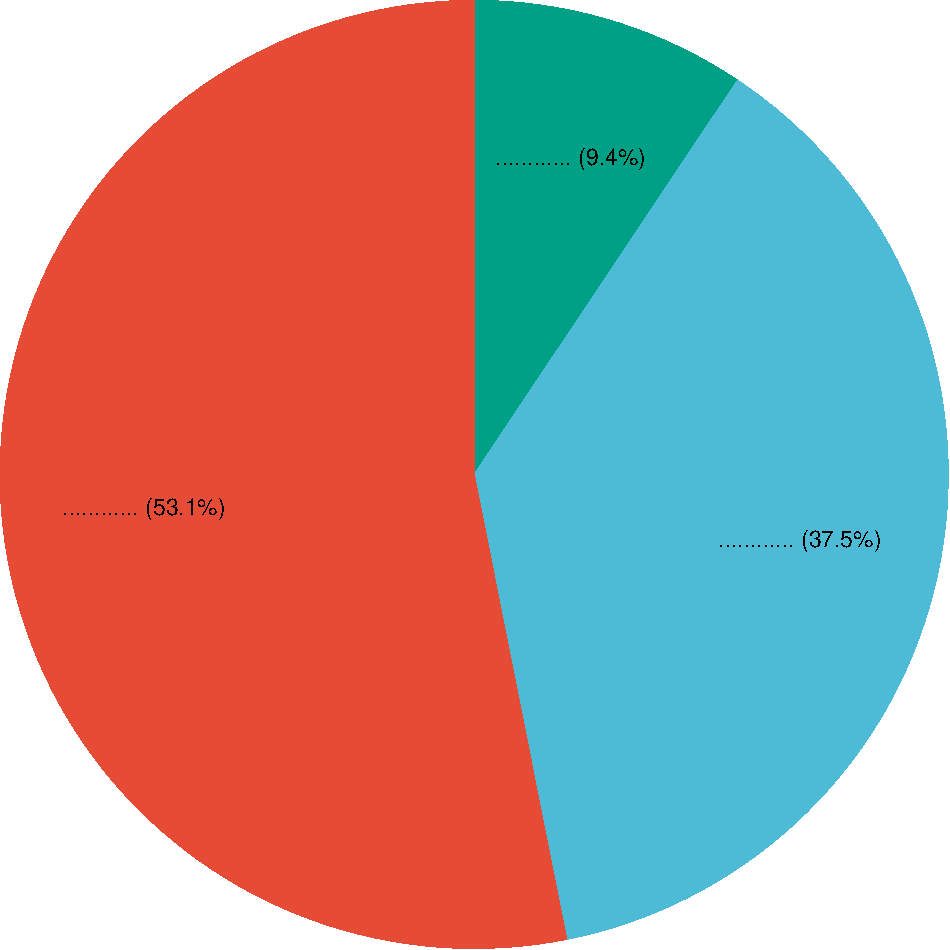
\includegraphics{slidy_6_year_files/figure-beamer/unnamed-chunk-2-1.pdf}
\end{frame}

\end{document}
